\section{Apêndice B -- Arquivos}

Todas as estruturas desta apostila vivem na memória principal: quando o programa termina, listas, árvores e tabelas desaparecem. Para que os dados sobrevivam, eles precisam ir para um \textbf{arquivo}, guardado no disco. Este apêndice mostra como ler e gravar arquivos em C++, primeiro como texto, que qualquer pessoa consegue abrir e editar, e depois em formato binário, com registros de tamanho fixo que podem ser acessados diretamente, a ideia na base dos bancos de dados.

\subsection{B.1 Fluxos de arquivo}

Em C++, um arquivo é tratado como um \textbf{fluxo} (\textit{stream}), exatamente como o teclado e a tela. A biblioteca \texttt{<fstream>} traz três tipos:

\begin{center}
\begin{tabular}{@{}p{0.22\linewidth}p{0.68\linewidth}@{}}
\toprule
\rowcolor{headergray}
\tblheader{Tipo} & \tblheader{Uso} \\
\midrule
\texttt{ofstream} & grava (\textit{output}); funciona como o \texttt{cout} \\
\rowcolor{rowgray} \texttt{ifstream} & lê (\textit{input}); funciona como o \texttt{cin} \\
\texttt{fstream} & lê e grava no mesmo arquivo \\
\bottomrule
\end{tabular}
\end{center}

Tudo o que você já sabe sobre \texttt{cin} e \texttt{cout} continua valendo: \texttt{<<} grava, \texttt{>>} lê um valor separado por espaços e \texttt{getline} lê uma linha inteira. O arquivo é aberto quando a variável é criada, com o nome do arquivo, e fechado automaticamente quando a variável deixa de existir. Também é possível fechá-lo antes, com \texttt{close}.

\subsection{B.2 Arquivos de texto}

O programa abaixo grava as notas de uma turma, uma por linha, e depois lê o arquivo de volta para calcular a média. Antes de usar um arquivo, sempre verifique se ele foi aberto: o nome pode estar errado, a pasta pode não existir ou o programa pode não ter permissão. O fluxo vira \texttt{false} quando algo dá errado, então basta testar \texttt{if (!saida)}.

\begin{codigo}
\begin{Verbatim}[breaklines=true, breaksymbolleft={}, fontsize=\footnotesize]
#include <fstream>
#include <string>

int main() {
    ofstream saida("notas.txt");   // cria (ou apaga o antigo)
    if (!saida) {
        cerr << "não foi possível criar notas.txt" << endl;
        return 1;
    }
    saida << "Ana 8.5" << endl;
    saida << "Bruno 5.0" << endl;
    saida << "Carla 9.0" << endl;
    saida.close();                 // grava tudo no disco

    ifstream entrada("notas.txt");
    string nome;
    double nota, soma = 0;
    int quantos = 0;
    while (entrada >> nome >> nota) {   // falso no fim
        soma += nota;
        quantos++;
    }
    cout << quantos << " notas, média " << soma / quantos << endl;
    // 3 notas, média 7.5
}
\end{Verbatim}
\end{codigo}

O laço \texttt{while (entrada >> nome >> nota)} é a forma correta de ler até o fim: a leitura em si é a condição, e ela falha quando não há mais dados. Uma armadilha comum é escrever \texttt{while (!entrada.eof())}: o fim do arquivo só é detectado \textbf{depois} de uma leitura que falhou, e a última linha acaba sendo processada duas vezes.

Abrir um \texttt{ofstream} apaga o conteúdo anterior do arquivo. Para \textbf{acrescentar} no fim, como em um diário ou um registro de eventos, abra com o modo \texttt{ios::app}. E, quando cada linha pode ter espaços, use \texttt{getline}:

\begin{codigo}
\begin{Verbatim}[breaklines=true, breaksymbolleft={}, fontsize=\footnotesize]
#include <fstream>
#include <string>

int main() {
    ofstream diario("diario.txt");          // começa vazio
    diario << "Segunda: estudei listas" << endl;
    diario.close();

    ofstream mais("diario.txt", ios::app);  // acrescenta
    mais << "Terça: estudei pilhas e filas" << endl;
    mais.close();

    ifstream leitura("diario.txt");
    string linha;
    int numero = 1;
    while (getline(leitura, linha)) {       // a linha inteira
        cout << numero++ << ": " << linha << endl;
    }
    // 1: Segunda: estudei listas
    // 2: Terça: estudei pilhas e filas

    ifstream inexistente("nao-existe.txt");
    if (!inexistente.is_open()) {
        cout << "arquivo não encontrado" << endl;
    }
}
\end{Verbatim}
\end{codigo}

\subsection{B.3 Arquivos CSV}

O formato \textbf{CSV} (\textit{comma-separated values}) guarda uma tabela em texto: cada linha é um registro, e os campos são separados por um caractere fixo. No Brasil, como a vírgula é usada nos números decimais, o separador costuma ser o ponto e vírgula, e é assim que as planilhas em português gravam. A primeira linha normalmente é um \textbf{cabeçalho} com os nomes das colunas.

Para ler cada campo, a linha inteira é lida com \texttt{getline} e depois quebrada com um \texttt{istringstream}, que trata o texto da linha como um fluxo. O \texttt{getline} aceita um terceiro parâmetro: o caractere em que deve parar.

\begin{codigo}
\begin{Verbatim}[breaklines=true, breaksymbolleft={}, fontsize=\footnotesize]
#include <fstream>
#include <sstream>    // istringstream
#include <string>
#include <vector>

struct Aluno {
    int matricula;
    string nome;
    double nota;
};

void salvarCsv(const string &arquivo,
               const vector<Aluno> &turma) {
    ofstream saida(arquivo);
    saida << "matricula;nome;nota" << endl;   // cabeçalho
    for (const Aluno &a : turma) {
        saida << a.matricula << ";" << a.nome << ";" << a.nota
              << endl;
    }
}

vector<Aluno> carregarCsv(const string &arquivo) {
    vector<Aluno> turma;
    ifstream entrada(arquivo);
    string linha;
    getline(entrada, linha);              // pula o cabeçalho
    while (getline(entrada, linha)) {
        istringstream campos(linha);
        string matricula, nome, nota;
        getline(campos, matricula, ';');  // lê até o ;
        getline(campos, nome, ';');
        getline(campos, nota);
        turma.push_back({stoi(matricula), nome, stod(nota)});
    }
    return turma;
}

int main() {
    salvarCsv("turma.csv", {{2031, "Ana Lima", 8.5},
                            {1987, "Bruno Reis", 5.0},
                            {2210, "Carla Dias", 9.0}});
    for (const Aluno &a : carregarCsv("turma.csv")) {
        cout << a.nome << " (" << a.matricula << "): " << a.nota
             << endl;
    }
    // Ana Lima (2031): 8.5
    // Bruno Reis (1987): 5
    // Carla Dias (2210): 9
}
\end{Verbatim}
\end{codigo}

As funções \texttt{stoi} e \texttt{stod} convertem texto em \texttt{int} e em \texttt{double}. Como os campos são separados pelo ponto e vírgula, e não por espaços, os nomes podem ter espaços sem problema. Um arquivo assim abre direto em uma planilha, o que faz do CSV um formato prático para trocar dados entre programas.

\subsection{B.4 Arquivos binários e acesso direto}

Um arquivo de texto só pode ser lido em sequência: para chegar ao milésimo aluno, é preciso ler os 999 anteriores, porque cada linha tem um tamanho diferente e não há como saber onde a milésima começa. A solução é gravar os dados em \textbf{formato binário}, com \textbf{registros de tamanho fixo}: se cada registro ocupa exatamente $t$ bytes, o registro $i$ começa no byte $i \times t$, e é possível pular direto para ele. É o mesmo princípio do vetor, em que \texttt{v[i]} é calculado a partir do endereço inicial.

\begin{center}
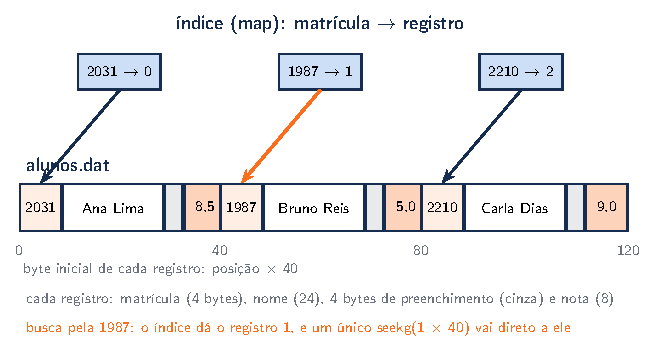
\includegraphics[width=0.95\linewidth,keepaspectratio]{imagens/apendice-b_registros.pdf}
\end{center}

Para que o registro tenha tamanho fixo, ele não pode conter \texttt{string} nem ponteiros, que guardam só um endereço da memória e não o conteúdo. O nome vai em um vetor de \texttt{char} com tamanho máximo definido. O registro é gravado com \texttt{write}, que copia os bytes da memória para o arquivo, e lido com \texttt{read}. As funções \texttt{seekg} e \texttt{seekp} posicionam a leitura e a gravação em um byte qualquer.

\begin{codigo}
\begin{Verbatim}[breaklines=true, breaksymbolleft={}, fontsize=\footnotesize]
#include <fstream>
#include <cstring>    // strncpy

struct Registro {      // tamanho fixo: vai direto para o disco
    int matricula;
    char nome[24];
    double nota;
};

Registro criar(int matricula, const char *nome, double nota) {
    Registro r{};                                // tudo zerado
    r.matricula = matricula;
    strncpy(r.nome, nome, sizeof(r.nome) - 1);   // sobra o '\0'
    r.nota = nota;
    return r;
}

int main() {
    const long T = sizeof(Registro);
    ofstream saida("alunos.dat", ios::binary);
    for (const Registro &r : {criar(2031, "Ana Lima", 8.5),
                              criar(1987, "Bruno Reis", 5.0),
                              criar(2210, "Carla Dias", 9.0)}) {
        saida.write(reinterpret_cast<const char *>(&r), T);
    }
    saida.close();

    fstream arquivo("alunos.dat",
                    ios::in | ios::out | ios::binary);
    Registro r;
    arquivo.seekg(2 * T);                     // direto ao 3º
    arquivo.read(reinterpret_cast<char *>(&r), T);
    cout << r.nome << ": " << r.nota << endl;  // Carla Dias: 9

    r.nota = 9.5;                             // corrige só ele
    arquivo.seekp(2 * T);
    arquivo.write(reinterpret_cast<const char *>(&r), T);

    arquivo.seekg(0, ios::end);               // vai para o fim
    cout << arquivo.tellg() / T << " registros de " << T
         << " bytes" << endl;   // 3 registros de 40 bytes
}
\end{Verbatim}
\end{codigo}

O \texttt{reinterpret\_cast<char *>} pede ao compilador para tratar o endereço do registro como uma sequência de bytes, que é o que \texttt{write} e \texttt{read} esperam. O registro tem 40 bytes, e não $4 + 24 + 8 = 36$: o compilador acrescenta 4 bytes de \textbf{preenchimento} antes da nota, para que o \texttt{double} fique em um endereço múltiplo de 8, que o processador acessa mais rápido. Por isso, sempre use \texttt{sizeof} em vez de somar os campos à mão. O \texttt{tellg} informa a posição atual em bytes; no fim do arquivo, é o tamanho dele.

\begin{center}
\begin{tabular}{@{}p{0.24\linewidth}p{0.33\linewidth}p{0.33\linewidth}@{}}
\toprule
\rowcolor{headergray}
\tblheader{} & \tblheader{Texto} & \tblheader{Binário} \\
\midrule
legível por pessoas & sim, em qualquer editor & não \\
\rowcolor{rowgray} acesso & sequencial & direto, com registros fixos \\
alterar um registro & reescrever o arquivo & gravar só aquele registro \\
\rowcolor{rowgray} portabilidade & alta & depende do tamanho dos tipos e da ordem dos bytes \\
tamanho & variável; números ocupam mais & fixo e compacto \\
\bottomrule
\end{tabular}
\end{center}

\subsection{B.5 Índices}

Com acesso direto, chegar ao registro número $i$ custa $O(1)$. Mas, na prática, ninguém procura ``o terceiro aluno do arquivo'', e sim ``o aluno de matrícula 1987''. Percorrer o arquivo inteiro comparando matrículas seria uma busca sequencial no disco, o que é muito lento. A solução é um \textbf{índice}: uma estrutura em memória que leva cada chave à posição do registro no arquivo. Ele pode ser uma árvore balanceada, como o \texttt{map}, ou uma tabela hash (Apêndice A). Uma consulta passa a ser uma busca no índice mais um único acesso ao disco.

\begin{codigo}
\begin{Verbatim}[breaklines=true, breaksymbolleft={}, fontsize=\footnotesize]
#include <fstream>
#include <map>
#include <cstring>    // strncpy

struct Registro {
    int matricula;
    char nome[24];
    double nota;
};

Registro criar(int matricula, const char *nome, double nota) {
    Registro r{};
    r.matricula = matricula;
    strncpy(r.nome, nome, sizeof(r.nome) - 1);
    r.nota = nota;
    return r;
}

int main() {
    const long T = sizeof(Registro);
    {
        ofstream saida("alunos.dat", ios::binary);
        Registro turma[] = {criar(2031, "Ana Lima", 8.5),
                            criar(1987, "Bruno Reis", 5.0),
                            criar(2210, "Carla Dias", 9.0)};
        for (const Registro &r : turma) {
            saida.write(reinterpret_cast<const char *>(&r), T);
        }
    }                                    // aqui a saída é fechada

    // monta o índice lendo o arquivo uma única vez
    ifstream arquivo("alunos.dat", ios::binary);
    map<int, long> indice;               // matrícula -> registro
    Registro r;
    long posicao = 0;
    while (arquivo.read(reinterpret_cast<char *>(&r), T)) {
        indice[r.matricula] = posicao++;
    }
    arquivo.clear();                     // tira o estado de fim

    // consulta: busca no índice e um único acesso ao arquivo
    auto it = indice.find(1987);
    if (it != indice.end()) {
        arquivo.seekg(it->second * T);
        arquivo.read(reinterpret_cast<char *>(&r), T);
        cout << r.nome << ": " << r.nota << endl;
        // Bruno Reis: 5
    }
    for (const auto &[matricula, reg] : indice) {
        cout << matricula << " -> " << reg << endl;
    }
    // 1987 -> 1, 2031 -> 0, 2210 -> 2 (o map mantém a ordem)
}
\end{Verbatim}
\end{codigo}

O par de chaves em volta da gravação cria um bloco: quando ele termina, a variável \texttt{saida} deixa de existir e o arquivo é fechado, antes de ser aberto para leitura. Depois que a leitura chega ao fim, o fluxo fica em estado de falha, e o \texttt{clear} é necessário para que o \texttt{seekg} volte a funcionar.

Os bancos de dados levam essa ideia muito mais longe. Eles guardam os registros em \textbf{páginas} de tamanho fixo no disco e usam como índice a \textbf{árvore B}, uma árvore balanceada como a AVL do Capítulo 5, mas com centenas de filhos por nó. Com tantos filhos, a árvore fica tão baixa que três ou quatro leituras de disco bastam para achar um registro entre milhões.

\begin{destaque}{Comparando com Python}
Em Python, a função \texttt{open} abre o arquivo, e o comando \texttt{with} garante que ele seja fechado ao final do bloco, mesmo que aconteça um erro no meio, o mesmo papel do bloco entre chaves do C++. Para CSV, o módulo \texttt{csv} cuida dos separadores e das aspas; para arquivos binários com registros fixos, o módulo \texttt{struct} converte valores em bytes.

\begin{codigo}
\begin{Verbatim}[breaklines=true, breaksymbolleft={}, fontsize=\footnotesize]
import csv

turma = [(2031, 'Ana Lima', 8.5), (1987, 'Bruno Reis', 5.0)]

with open('turma.csv', 'w', newline='', encoding='utf-8') as arq:
    escritor = csv.writer(arq, delimiter=';')
    escritor.writerow(['matricula', 'nome', 'nota'])
    escritor.writerows(turma)

with open('turma.csv', encoding='utf-8') as arq:
    for linha in csv.DictReader(arq, delimiter=';'):
        print(linha['nome'], float(linha['nota']))
# Ana Lima 8.5
# Bruno Reis 5.0
\end{Verbatim}
\end{codigo}

O \texttt{DictReader} usa o cabeçalho para dar nome aos campos de cada linha. Indique sempre o \texttt{encoding='utf-8'}: sem ele, o Python usa a codificação padrão do sistema, e nomes com acentos podem sair trocados ao abrir o arquivo em outro computador.
\end{destaque}

\subsection{Erros Comuns}

\begin{itemize}
  \item \textbf{Não verificar se o arquivo abriu.} Com um nome errado, todas as leituras falham em silêncio e o programa segue com variáveis vazias.
  \item \textbf{Usar \texttt{while (!arquivo.eof())}.} O fim só é detectado depois de uma leitura que falhou, e o último registro é processado duas vezes. Use a própria leitura como condição.
  \item \textbf{Apagar um arquivo sem querer.} Abrir um \texttt{ofstream} apaga o conteúdo anterior. Para acrescentar, use \texttt{ios::app}.
  \item \textbf{Misturar \texttt{>>} e \texttt{getline}.} O \texttt{>>} deixa a quebra de linha no fluxo, e o \texttt{getline} seguinte lê uma linha vazia. Leia tudo com \texttt{getline}, ou descarte o resto da linha antes.
  \item \textbf{Esquecer o \texttt{ios::binary}.} No Windows, o modo texto troca as quebras de linha ao gravar e ao ler, o que corrompe os bytes de um registro binário.
  \item \textbf{Gravar \texttt{string} ou ponteiros em binário.} O \texttt{write} grava o endereço que está dentro deles, e não o texto. Ao ler de volta, em outra execução, esse endereço não significa nada.
  \item \textbf{Calcular o tamanho do registro somando os campos.} O preenchimento muda o total. Use \texttt{sizeof}.
  \item \textbf{Esquecer o \texttt{clear} depois de chegar ao fim.} O fluxo fica em estado de falha e ignora os \texttt{seekg} e \texttt{read} seguintes.
\end{itemize}
